%Ne pas numéroter cette partie
\part*{Annexes}
%Rajouter la ligne "Annexes" dans le sommaire
\addcontentsline{toc}{part}{Annexes}

\begin{center}\textbf{Vocabulaire}\end{center}

\begin{itemize}
\item \textsc{Panel}: Élément graphique de Unity 5 représenté par un panneau configurable sur lequel placer des éléments héritant de la classe UI.
\item \textsc{UI}: \textit{User Interface}, classe fournie par Unity comprenant les Panels, boutons, textes, éléments d'interface graphique. 
\item \textsc{Drag \& Drop}: Glisser-déposer en français, manière de gérer une interface en permettant le déplacement de certains éléments vers d'autres conteneurs. 
\item \textsc{Tile}: Tuile en français, correspond à une case du jardin.
\end{itemize}

\begin{center}\textbf{Grammaire pour la vérification syntaxique}\end{center}

\begin{center}
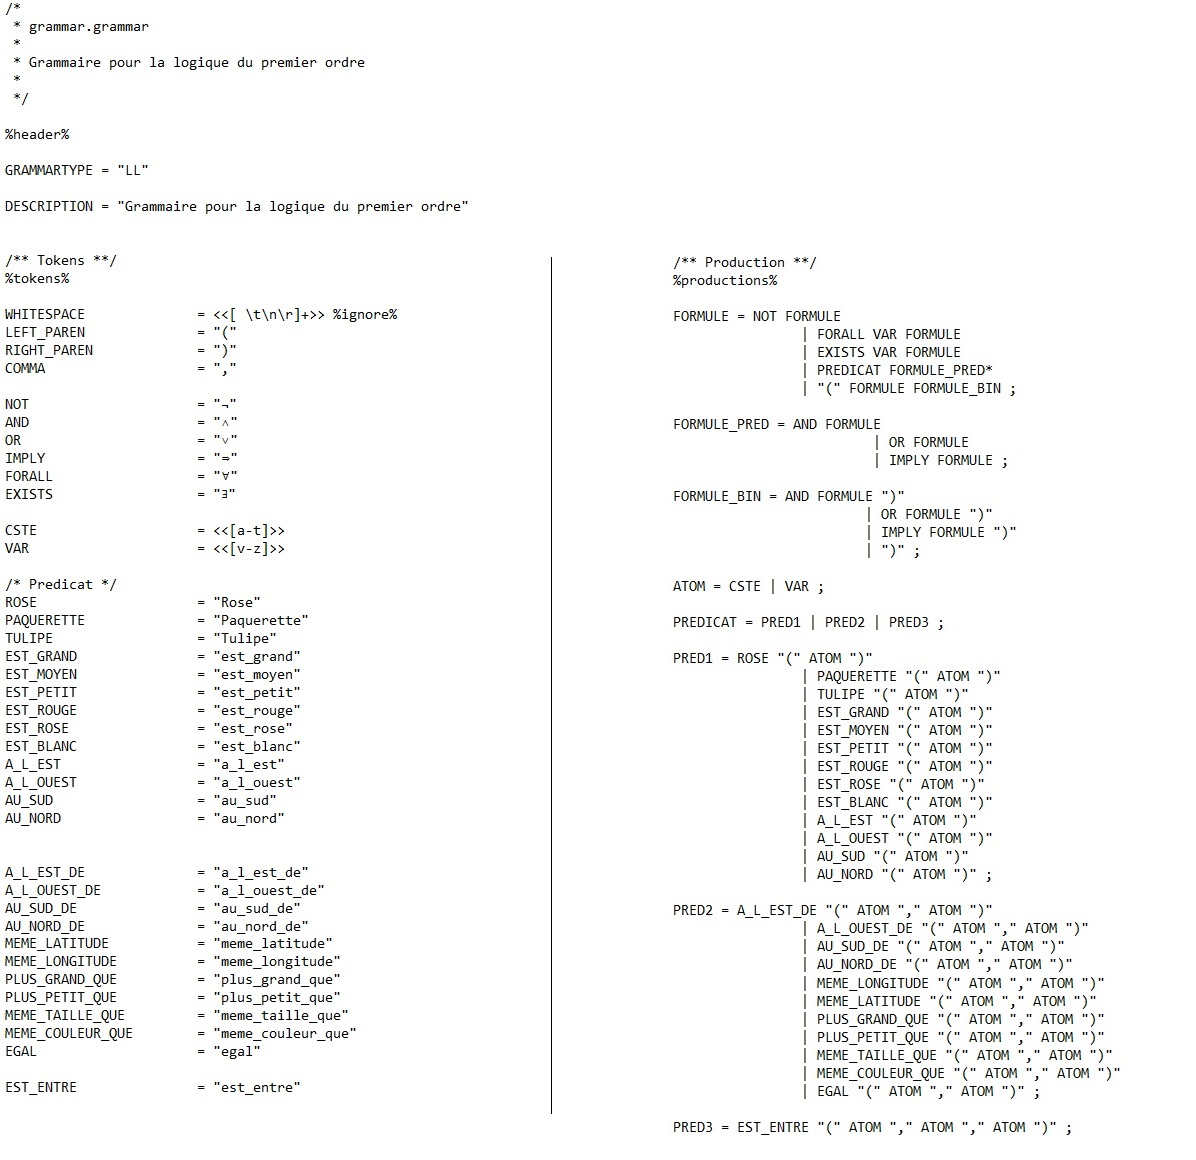
\includegraphics[scale=0.5]{annexes/grammaire.jpg}
\end{center}